\documentclass{book}
\usepackage[allcolors=true]{hyperref}
\usepackage{graphicx}
\usepackage{amsmath,amsfonts,amsthm,amssymb}
\usepackage{tikz, xcolor}

%\newcommand\bg[2]{
%\begin{center} \fcolorbox{white}{BGgris}{\parbox{.9\linewidth}{\begin{large} %\textit{#1} \end{large} \\ #2 }}
%\end{center}}

\begin{document}

\chapter{L'équation de Schrödinger - Suite}\label{chap:chap3}



\section{Equation de Schrödinger en potentiel carré}
Dans cette sections nous traitons plusieurs cas de potentiels, qui ont pour point commun de répondre à la définition de "potentiel carré" présentée à la section suivante. Nous pouvons les organiser de la sorte :
\begin{itemize}
  \item Puits de potentiel : on mettra en évidence la présence \textbf{d'états liés}
    \begin{itemize}%[label = $\star$]
      \item Infini
      \item Fini
    \end{itemize}
  \item Marche de potentiel : on verra l'effet tunnel
\end{itemize}
\subsection{Définition d'un potentiel carré} \label{ch2-subsection-Definition_pot_carre}
Un potentiel carré est un potentiel présentant des discontinuités sous la forme de "marches" \footnote{Synonymes : potentiel en marche d'escalier, potentiels continus par morceaux}. Une grandeur physique ne pouvant pas présenter de discontinuité en réalité, le potentiel carré en est néanmoins souvent une excellente \textbf{approximation}.




\begin{figure}[h]
\centering
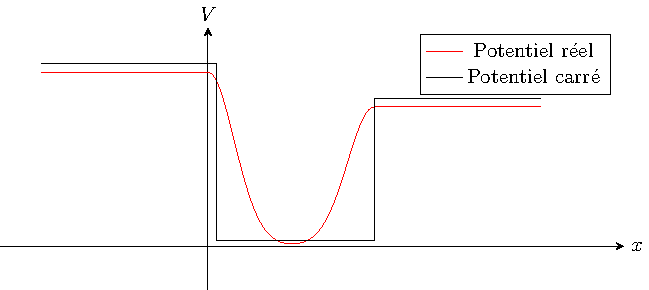
\includegraphics[width=0.5\linewidth]{images/pot_carre.pdf}
\caption{Illustration d'un puits de potentiel carré en comparaison avec un puits de potentiel réel.}
\label{fig:potentiel_carre}
\end{figure}


%*************

Un puits de potentiel est une région de l'espace où le potentiel atteint un minimum. Cette notion existe en mécanique classique, alors nous pourrions parler ici de puits quantique pour parler d'un puits dont les dimensions sont si petites qu'elles ne peuvent nous protéger d'entrer dans la mécanique quantique (cf. début de section). Mais nous garderons la dénomination de "puits de potentiel" car ce document ne concerne que la mécanique quantique. \\


\subsection{Puits de potentiel infini}
Un puits de potentiel infini a des discontinuités tendant vers l'infini. Il peut s'apparenter à une "boîte", c'est pourquoi on parle souvent de "particule dans une boîte". Par ailleurs, intuitivement, comme une particule ne peut pas exister dans une région où règne un potentiel infini, la particule sera \textbf{confinée dans une boîte}.



\begin{figure}[h]
\centering
%\scalebox{1}{%\documentclass{standalone}
%\usepackage{tikz, xcolor, amsmath}

%\begin{document}
\begin{tikzpicture}
\draw[thick, ->] (-1,0) --+ (8,0) ;
\draw[thick, ->] (0,-0.2) --+ (0,5) ;
\draw[red] (2,-0.1) --+ (0,4) ;
\draw[red, dashed] (2, 4) --+ (0,1) ;
\draw[red, dashed] (5, 4) --+ (0,1) ;
\draw[red] (5,-0.1) --+ (0,4) ;
\node at (2,-0.3) {0} ;
\node at (5,-0.3) {$L$} ;
\node at (8, 2.5) {$\boxed{V(x) = \begin{cases}
+\infty &x\leq 0 \\
0 & 0 < x < L \\
+\infty &x \geq L 
\end{cases}}$
} ;
\end{tikzpicture}
%\end{document}}
\caption{Puits de potentiel.}
\label{fig:puits_potentiel}
\end{figure}

%*************

\subsubsection{Résolution de l'équation \eqref{eq:schrodinger_stationnaire} dans un puits en 1D}
L'équation de Schrödinger se réécrit encore 



\begin{equation}\label{eq:schrodinger_1D}
i \hbar \dfrac{\partial }{\partial t} \; \psi(x, t) \; = \; -\dfrac{\hbar ^2}{2m} \; \dfrac{ \partial ^2}{\partial x^2} \psi(x, t) \; + \; V(x) \psi(x,t)
\end{equation}
où $V(x)$ suit la figure \ref{fig:puits_potentiel}.
La séparation des variables s'écrit :
$$\psi(x,t) = \chi(t) \varphi(x)$$ et la partie temporelle se résout facilement.
$$\chi(t) = \chi_0 \; e^{-iE\; t/\hbar}$$
La partie spatiale elle s'écrit :
$$
\left(-\dfrac{\hbar ^2}{2m} \dfrac{ d ^2}{d x^2 }  + V(x)\right) \varphi(x) \; = \; E  $$
Le problème du puits de potentiel ne demande pas que de résoudre cette équation différentielle. En effet, c'est un problème avant tout \textbf{physique}, et il impose naturellement des conditions aux bords. Nous savons que la particule ne peut pas se trouver aux murs du potentiel ($x=0$ ou $x=L$) ni à l'intérieur des murs (en dehors de $]0,L[$) car elle ne peut pas exister dans une zone où le potentiel est infini. Alors, nous avons les conditions aux bords suivantes :
$$\text{Conditions aux bords : }\quad 
\left\{
  \begin{array}{ll}
    \varphi(0) &= 0 \\
    \varphi(L) &= 0 \\
  \end{array}
\right.
$$

\subsubsection{Quantification de l'énergie}
De manière complète, l'équation différentielle pour la partie spatiale de l'équation s'écrit 
$$\left \{ \begin{array}{ll}
  \left(-\dfrac{\hbar ^2}{2m} \dfrac{ d ^2}{d x^2 }  + V(x)\right) \varphi(x) \; &= \; E \\ \strut \\
  \text{Conditions au bord : } \quad \varphi(0) &= \varphi(L) = 0
  \end{array} \right. \; . $$


Nous allons nous intéresser qu'au cas où la particule est entre $0$ et $L$, car elle ne peut pas exister dans une zone où le potentiel est infini. \textbf{Dans le cas où} $0<x<L$, nous avons donc un potentiel nul et les conditions aux bords à respecter, d'où :
\begin{equation}
\begin{array}{lrl}
& -\dfrac{\hbar ^2}{2m} \dfrac{ d ^2}{d x^2 } \varphi(x) &= E \varphi (x) \\
&\text{\small (en posant)} \quad k &= \sqrt{\dfrac{2mE}{\hbar ^2}} \\
\iff & \varphi(x) &= \alpha \sin(kL) + \beta\cos(kL) \\ \strut \\
&\text{CB} \;  &:  \; \left\{ \begin{array}{lll}
\varphi(0) &= 0 \quad \Rightarrow \quad \beta &= 0 \\
\varphi(L) &= 0 \quad \Rightarrow \quad kL &= n\pi \\
\end{array}\right. \\ \strut \\
&\Rightarrow \quad k_n &= \dfrac{n\pi}{L}
\end{array}
\end{equation}
Les conditions aux bords imposent donc une condition sur $k_n$, et \textit{a fortiori} sur l'énergie aussi, par la définition de $k_n$. Ainsi, par la définition du problème du puits de potentiel, la particule confinée au sein du puits ne peut avoir que certains états d'énergie. L'énergie est alors dite quantifiée.
\begin{equation}\label{eq:quantification_energie}
\boxed{\text{Quantification de l'énergie : } \quad E_n = \dfrac{\hbar ^2 \pi ^2 n ^2}{2m \; L^2}}
\end{equation}

\subsubsection{Normalisation des solutions $\psi_n$}
De retour à l'équation de Schrödinger avec la forme générale de $\varphi(x)$, avec $\beta = 0$ et $\alpha$ indéterminé, la solution à \eqref{eq:schrodinger_1D} s'écrit pour un niveau d'énergie $E_n$ comme produit de $\varphi_n(x)$ et de $\chi_n(t)$ :
$$\psi_n(x,t) = A \; \underbrace{e^{-i \dfrac{E_n}{\hbar}t}}_{\chi_n(t)} \; \underbrace{\sin\left(\dfrac{n\pi}{L} \; x\right)}_{\varphi_n(x)} \; ,$$
avec un coefficient $A \in \mathbb{C}$. Ce coefficient multiplie la fonction d'onde et nous permettra d'avoir une fonction d'onde $\psi_n$ \textbf{normée} pour chaque état d'énergie $E_n$, et ce en tout temps $t$. Ceci est d'une importance particulière qui sera rappelée au chapitre 4. La fonction $\psi_n$ étant à valeurs complexes, la norme utilisée sera celle des fonctions à valeurs complexes. Ainsi, avoir $|\psi_n|^2 = 1$ revient à imposer, vu que la fonction prend des valeurs nulles en dehors de $]0,L[$, 
$$
\int_{-\infty} ^{+\infty} |\psi_n(x)|^2 \; dx = \int_{0} ^{L}\left| A \; e^{-i \dfrac{E_n}{\hbar}t} \; \sin \left(\dfrac{n\pi}{L}\right)\;\right|^2 dx =  1
\; .
$$
Or, le module d'une exponentielle purement imaginaire est égal à $1$, et le module d'un produit est égal au produit des modules : ainsi, vu que $A$ est indépendant de $x$, il peut sortir de l'intégrale. Nous avons alors
$$
\int_{0} ^{L} \sin\left(\dfrac{n\pi}{L}\right)^2 dx = \dfrac{1}{|A|^2}
$$
Ce qui peut s'évaluer en utilisant la formule de Carnot :
$$
\sin(\alpha)^2 = \frac{1 }{2}(1-\cos(2\alpha))
$$
en 
$$
\int_{0} ^{L} \dfrac{1 }{2}\left(1-\cos\left(2\; \dfrac{n\pi}{L}\right)\right) dx = \dfrac{1}{|A|^2}
$$
$$
\iff |A| = \sqrt{\dfrac{2}{L}}
$$
Nous avons donc que la solution d'énergie $E_n$ a la forme
$$\psi_n(x,t) = A \; e^{-i \dfrac{E_n}{\hbar}t} \; \sin\left(\dfrac{n\pi}{L} \; x\right) \; ,$$
avec $A$ un coefficient complexe de norme $(2/L)^{1/2}$. Nous pouvons, sans perdre de généralité, \textit{choisir} $A$ comme étant \textbf{réel et positif}, c'est-à-dire \textit{choisir sa phase}. Un choix de phase différent n'impacte en rien les propriétés physiques de l'état.
$$\psi_n(x,t) = \sqrt{\dfrac{2 }{L}} \; e^{-i \dfrac{E_n}{\hbar}t} \; \sin\left(\dfrac{n\pi}{L} \; x\right) \; ,$$

\subsubsection{Solution générale}
Pour obtenir la solution générale, il convient de sommer sur les états d'énergie :

\begin{equation}\label{eq:chap3-puits_fourier}
  \psi(x,t) = \sum_{n=1} ^{+\infty} c_n \psi_n(x,t)  = \sum_{n=1} ^{+\infty} c_n \sqrt{\dfrac{2 }{L}} \; e^{-i \dfrac{E_n}{\hbar}t} \; \sin\left(\dfrac{n\pi}{L} \; x\right)
\end{equation}
où les coefficients $c_n$ sont tels que 
$$
\sum_{n=1} ^{\infty} |c_n|^2 = 1
$$
pour que la solution générale soit normée. 

\subsubsection{Lien avec les séries de Fourier}
Notons que la solution \eqref{eq:chap3-puits_fourier} ressemble à un développement en série de Fourier sur l'espace des fonctions $\varphi_n$ (la partie spatiale de $\psi_n$) si elles forment une base orthonormée. Pour cela, il faut que pour deux niveaux d'énergie différents $n, n' \in \mathbb{N}$ :
$$
\int_0 ^L \varphi_{n_1}(x) \varphi_{n_2}^*(x) \; dx = \delta_{n\; n'} \; .
$$
Notons bien qu'ici on évalue le fait que les $\varphi_n$ soient orthonormées, car on veut qu'elles constituent notre base pour le développement en série de Fourier. Nous ne nous intéressons pas aux $\chi_n$ ! Evaluons le membre de gauche. Les $\varphi_n$ sont réelles, donc la conjugaison peut se retirer.
$$
\int_0 ^L \varphi_n(x) \varphi_{n'}(x) = 
\int_0 ^L \dfrac{2 }{L} \sin\left(\dfrac{n\pi}{L} x\right)\sin\left(\dfrac{n'\pi}{L} x\right) \; dx = \delta_{n\; n'}
$$
car le système de fonctions $\left\{\sin\left(\dfrac{n\pi}{L} x\right)\; ; n\in\mathbb{N}_0\right\}$ est orthogonal sur $[0,L]$ (voir un cours sur les Séries de Fourier pour la justification).

\subsubsection{Conclusion}
Les conclusions que nous pouvons tirer pour la résolution de l'équation de Schrödinger dans le cas d'un puits de potentiel de largeur $L$ sont :
\begin{itemize}
  \item Commencer par une séparation des variables : l'énergie de chaque état est contenue dans l'\textbf{évolution temporelle} $\chi_n$.
  \item La physique du problème impose des conditions aux bords sur la partie spatiale, et ceci mène à une \textbf{quantification de l'énergie} \eqref{eq:quantification_energie}.
  \item Une fois les deux parties obtenues, spatiale et temporelle, les multiplier donne la solution pour un état d'énergie. Cette solution est à \textbf{normer} (voir chapitre 4).
  \item Une fois normées, les fonctions peuvent se sommer pour constituer la solution générale. Ici, la chose importante à remarquer est que l'espace des fonctions $\varphi_n$ calculées lors de la séparation des variables constitue en fait un \textbf{système orthonormé} et donc la solution générale \eqref{eq:chap3-puits_fourier} peut se comprendre comme le \textbf{développement en série de Fourier} de $\psi$.
\end{itemize}

\subsection{Puits de potentiel fini}
Un puits de potentiel fini est un cas assez basique de potentiel carré. Une image vaut mieux que mille mots :

\begin{figure}[h]
  \centering
  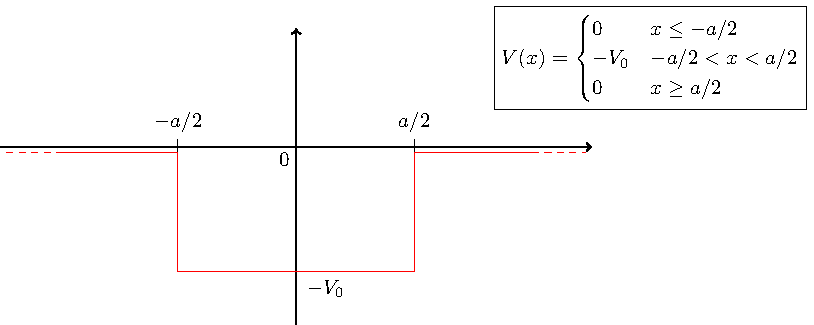
\includegraphics[scale=0.8]{images/puits_potentiel_fini.pdf}
  \caption{Illustration d'un puits de potentiel fini de largeur $a$ et de profondeur $V_0$.}
  \label{fig:chap2-potentiel_fini}
\end{figure}



Écrivons la partie spatiale de l'équation de Schrödinger et observons qu'une équation avec $V$ fonction de $x$ peut se réécrire en 3 équations avec $V$ constant : les 3 zones $x\leq -a/2$, $-a/2\leq x\leq a/2$, et $a/2 \leq x$.

%************

\begin{equation}
  -\dfrac{\hbar^2}{2m} \partial_x ^2 \varphi = (E-V(x)) \varphi 
  \quad \Rightarrow \quad \ \left\{ 
    \begin{array}{lll}
      \text{Zone I} & V = 0 & -\dfrac{\hbar^2}{2m} \partial_x ^2 \varphi = E \varphi \\
      \text{Zone II} & V = -V_0 & -\dfrac{\hbar^2}{2m} \partial_x ^2 \varphi = (E+V_0) \varphi \\
      \text{Zone III} & V = 0 & -\dfrac{\hbar^2}{2m} \partial_x ^2 \varphi = E \varphi \\
    \end{array}
    \right. 
  \end{equation}
  Ces équations sont simples à résoudre, et donnent :
  \begin{align}
    \varphi_{\mathrm{I}}(x) &= B_1 e^{\rho x} + B' _1 e^{-\rho x} \\
    \varphi_{\mathrm{II}}(x) &= A_2 e^{ik x} + A' _2 e^{-ik x} \\
    \varphi_{\mathrm{III}}(x) &= B_3 e^{\rho x} + B' _3 e^{-\rho x} 
  \end{align}
  où
  \begin{align}
    \rho &= \sqrt{-\dfrac{2mE}{\hbar}} \quad \in \mathbb{C} \\
    k &= \sqrt{\dfrac{2m(E+V_0)}{\hbar}} \quad \in \mathbb{R} \\
  \end{align}
  Les coefficients apparaissant dans la forme de la fonction d'onde doivent être déterminés. C'est la physique du problème qui nous les offira. Les conditions que doit remplir une fonction d'onde sont :
  \begin{itemize}
    \item $\varphi$ continue 
    \item $\varphi'$ continue
  \end{itemize}
  Et ce, même si le potentiel est discontinu. Dans le cas d'un puits de potentiel fini, il n'y a pas d'autres conditions particulières à imposer. La première impose $B_1' = B_3 = 0$. \\
  
  Les deux suivantes imposent ensembles :
  \begin{equation}\label{eq:chap3-pot_carre_conditions}
    \left(\dfrac{\rho - ik}{\rho + ik} \right) ^2 = e ^{2ika}
  \end{equation}
  \begin{proof}
    Nous devons avoir $\varphi$ et $\partial_x \varphi$ continues, donc particulièrement en $x=-a/2$ et $x=a/2$.

    $$
    \begin{array}{ll}
      x=-a/2 \; :& \left\{
        \begin{array}{ll}
          B_1 \; e^{-\rho\; a/2} &= A_2 e^{-ik\; a/2} + A_2 ' e^{ik\; a/2} \\
          \strut \\
          \rho B_1 e^{-\rho\; a/2} &= ik\left(A_2e^{-ik\; a/2} - A_2 ' e^{ik\; a/2}\right)
        \end{array}
      \right. \\
      \strut \\
      \iff& \left\{
        \begin{array}{ll}
          A_2 &= e^{(-\rho + ik)} a/2 \; \dfrac{\rho + ik}{2ik} B_1 \\
          A_2 ' &= e^{-(\rho + ik)} a/2 \; \dfrac{\rho - ik}{2ik} B_1 \\
        \end{array}
      \right. \\
    \end{array}
    $$

    $$
    \begin{array}{ll}
      x=a/2 \; :& \left\{
        \begin{array}{ll}
          B_3 ' \; e^{\rho\; a/2} &= A_2 e^{ik\; a/2} + A_2 ' e^{-ik\; a/2} \\
          \strut \\
          -\rho B_3 ' e^{\rho\; a/2} &= ik\left(A_2e^{ik\; a/2} - A_2 ' e^{-ik\; a/2}\right)
        \end{array}
      \right. \\
      \strut \\
      \iff& \left\{
        \begin{array}{ll}
          A_2 &= e^{(-\rho + ik)} a/2 \; \dfrac{\rho + ik}{2ik} B_1 \\
          A_2 ' &= e^{-(\rho + ik)} a/2 \; \dfrac{\rho - ik}{2ik} B_1 \\
        \end{array}
      \right. \\
    \end{array}
    $$
  \end{proof}
  La condition \eqref{eq:chap3-pot_carre_conditions} possède deux solutions.
  \begin{enumerate}%[label = (\roman*)]
    \item $\dfrac{\rho - ik}{\rho + ik} = -e^{ika}$ \\
    Nous avons dans le membre de gauche un quotient de deux nombres complexes $z_1/z_2$. Le module de ce nombre est $\bar z_1/\bar z_2$ (soit 1 ici) et sa phase est $\phi(z_1) - \phi(z_2)$ où $\phi(z) = b/a$. Alors, le membre de gauche est de module 1 et de phase $-2\times \arctan(k/\rho)$. Grâce à ça nous pouvons écrire :
    \begin{eqnarray*}
      1\times e^{-2i\arctan(k/\rho)} &=& - e^{ika} \\
      \iff \dfrac{k}{\rho} &=& \tan\left(\dfrac{ka}{2}\right)
    \end{eqnarray*}
    
    Posons à présent $k_0 = \sqrt{k^2 + \rho ^2}$ et exploitons la relation trigonométrique $$\dfrac{1}{\cos ^2(x)} = \tan^2(x) +1$$ en l'appliquant à $ka/2$. Il vient :
    $$\dfrac{1}{\cos ^2\left(\dfrac{ka}{2}\right)} = \tan^2\left(\dfrac{ka}{2}\right) +1  = \dfrac{k^2 + \rho^2}{k^2} = \left(\dfrac{k}{k_0}\right)^2$$
    La solution s'obtient donc en résolvant le système d'équations suivant :
    \begin{equation}
      \left\{ \begin{array}{ll}
        \left| \cos \left(\dfrac{ka}{2}\right)\right| &= \dfrac{k}{k_0} \\
        \tan \left(\dfrac{ka}{2}\right) &>0
      \end{array}\right.
    \end{equation}
    
    qui peut se résoudre graphiquement en traçant les intersections de la droite $k/k_0$ avec des arcs de cosinusoïdes. \\
    \item $\dfrac{\rho - ik}{\rho + ik} = e^{ika}$ \\
    
    Par une démarche similaire à la précédente, les résultats sont aussi similaires. Nous avons :
    \begin{equation}
      \left\{ \begin{array}{ll}
        \left| \sin \left(\dfrac{ka}{2}\right)\right| &= \dfrac{k}{k_0} \\
      \tan \left(\dfrac{ka}{2}\right) &<0
    \end{array}\right.
  \end{equation}
\end{enumerate}
La résolution de cette équation de Schrödinger passe par l'obtention de ces coefficients. Comme on vient de le voir, il est possible de ne pas en obtenir une expression directe (résolution analytique), mais une résolution \textbf{graphique} permet d'obtenir les états liés sous le potentiel en question. Par exemple, ici, il suffit d'observer les intersections entre les arcs de (co-)sinusoïdes et la droite $k/k_0$, et ne considérer que celles qui ont un $k$ tel que la tangente est positive (pour les cosinusoïdes) ou négative (sinusoïdes). 

\begin{figure}[h]
  \centering
  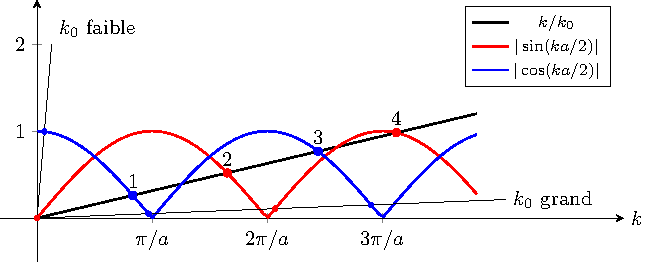
\includegraphics{images/chap2-puits_fini_solutions.pdf}
  \caption{Résolution graphique d'une équation de Schrödinger. Partant de l'équation, une séparation a été faite en 3 zones, donnant des états d'énergie possibles au sein de la barrière (états \textbf{liés}) caractérisés par le nombre $k$. Les énergies des états liés sont ceux dont le $k$ donne un point d'intersection sur la figure.}
\end{figure}

De ce graphe nous tirons l'information suivante.
Dépendant de la pente $1/k_0$, un certain nombre d'états liés peuvent exister. Particulièrement, lorsque $1/k_0  \geq A/(\pi a)$ (autrement dit $k_0 \leq \pi a$), alors la particule n'a qu'un seul état lié au potentiel. De manière générale, si $(n-1)\pi/a \leq k_0 \leq n\pi/a$, la particule aura $n$ états liés.



\subsection{Marche de potentiel}
Une marche de potentiel est similaire au puits fini mais avec un potentiel positif. Ce potentiel s'oppose donc à l'énergie de la particule et c'est pour cette raison qu'on parle souvent de "barrière de potentiel".

\begin{figure}[h]
  \centering
  \scalebox{1.2}{\documentclass{standalone}
\usepackage{tikz, xcolor, amsmath}
\begin{document}
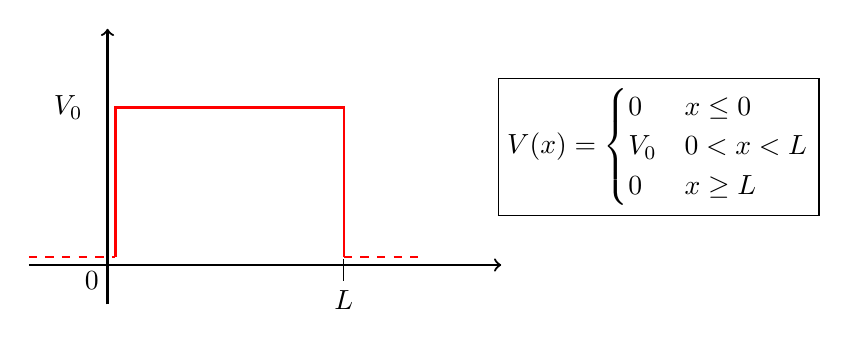
\begin{tikzpicture}
    \draw[thick, ->] (-1,0) --+ (6,0) ;
    \draw[thick, ->] (0,-0.5) --+ (0,3.5) ;
    \draw[thick, red] (0.1, 0.1) -- (0.1, 2) -- (3, 2) -- (3, 0.1) ;
    \draw[thick, red, dashed] (-1, 0.1) -- (0.1, 0.1) ;
    \draw[thick, red, dashed] (3, 0.1) -- (4, 0.1) ;
    \draw (3, 0.07) -- (3, -0.2) node[below] {$L$} ;
    \node at (-0.5, 2) {$V_0$} ;
    \node at (7, 1.5) {$\boxed{V(x) = \begin{cases}
    0 &x\leq 0 \\
    V_0 & 0 < x < L \\
    0 &x\geq L \\
    \end{cases}}$
    } ;
    \node at (-0.2, -0.2){$0$};
    
\end{tikzpicture}
\end{document}}
  \caption{Illustration d'un puits de potentiel fini de largeur $a$ et de profondeur $V_0$.}
  \label{fig:chap2-marche_potentiel}
\end{figure}

\subsubsection{Comparaison avec la mécanique classique}
%\begin{wrapfigure}{r}{0.6\textwidth}
\begin{figure}%{r}{0.6\textwidth}
  \centering
  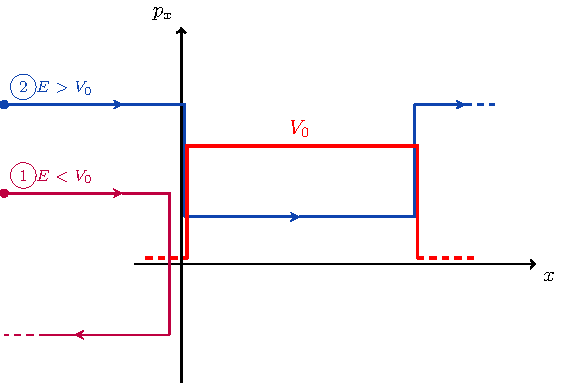
\includegraphics[width=.9\linewidth]{images/marche_potentiel_classique.pdf}
  \caption{Impact sur la trajectoire dans l'espace des phases (axes : position et impulsion, vitesse constante = ligne droite) d'une particule qui passe à travers une marche de potentiel.}
  \label{fig:ch2-marche_potentiel_classique}
  \end{figure}
%\end{wrapfigure}

Etudier ce cas est très intéressant car une marche de potentiel en physique quantique donne un résultat extrêmement différent de la physique classique. En effet, en physique classique, une particule arrivant avec une énergie inférieure à $V_0$ rebondira. Avec une énergie supérieure à $V_0$, elle sera ralentie dans le potentiel (potentiel constant veut dire "force nulle" donc la particule a quoi qu'il arrive une vitesse constante) et repart avec sa vitesse initiale. Avec une énergie $E= V_0$, elle s'arrête.  Ces discussions sont reprises sur la figure ci-contre. \\

Pour ce qui est de la physique quantique, il faut passer par une résolution de l'équation de Schrödinger. Comme pour le puits de potentiel, écrivons l'équation dans les différentes zones et écrivons les conditions de raccordement. Notons que la forme des solutions obtenues diffère selon si $E>$ ou $< V_0$.
\subsubsection{Résolution lorsque $E > V_0$}
Nous pouvons poser le nombre 
$$k_2 = \sqrt{\dfrac{2m(E-V_0)}{\hbar}}$$
de sorte à ce qu'il soit réel, et séparer en zones comme fait pour le puit de potentiel fini.
\begin{equation}
  -\dfrac{\hbar^2}{2m} \partial_x ^2 \varphi = (E-V(x)) \varphi 
  \quad \Rightarrow \quad \ \left\{ 
    \begin{array}{lll}
      \text{Zone I} & V = 0 & -\dfrac{\hbar^2}{2m} \partial_x ^2 \varphi = E \varphi \\
      \text{Zone II} & V = V_0 & -\dfrac{\hbar^2}{2m} \partial_x ^2 \varphi = (E-V_0) \varphi \\
      \text{Zone III} & V = 0 & -\dfrac{\hbar^2}{2m} \partial_x ^2 \varphi = E \varphi \\
    \end{array}
    \right. 
  \end{equation}
  Ces équations sont simples à résoudre, et donnent :
  \begin{align}
    \varphi_{\mathrm{I}}(x) &= A_1 e^{k_1 x} + A' _1 e^{-k_1 x} \\
    \varphi_{\mathrm{II}}(x) &= A_2 e^{ik_2 x} + A' _2 e^{-ik_2 x} \\
    \varphi_{\mathrm{III}}(x) &= A_3 e^{k_1 x} + A' _3 e^{-k_1 x} 
  \end{align}
  où
  $$
    k_1 = \sqrt{-\dfrac{2mE}{\hbar}} \quad \in \mathbb{C} 
  $$
Les considérations physiques et les conditions de raccord impliquent encore des relations entre les coefficients. Notamment :

\begin{align}
  A_1 &= \left[\cos(k_2 L) - i \; \dfrac{k_1 ^2 + k_2 ^2}{2k_1k_2} \; \sin(k_2L) \right] e^{ik_1L}A_3 \\
  A_1 ' &= i \; \dfrac{k_2 ^2 - k_1 ^2}{2k_1 k_2}\; \sin(k_2L) \; e^{ik_1L} A_3
\end{align}

Une manière d'interpréter la physique du système est d'observer les ainsi nommés \textbf{coefficients de transmission et de réflexion}. Comme leur nom l'indique, ces coefficients quantifient la probabilité que la particule traverse la barrière et la probabilité qu'elle soit réfléchie en la rencontrant. Ainsi, ces coefficients seront toujours exprimés comme un rapport où le dénominateur est $A_1$ : le coefficient de la partie de la fonction d'onde qui symbolise une particule se dirigant vers les $x>0$ avec un nombre d'onde $k_1$, soit l'état initial de la particule.\\

De là, la réflexion de la particule sera lue dans le coefficient $A_1'$, qui correspond à une fonction d'onde dans la zone 1 de nombre d'onde $k_1$ se propageant vers la gauche.

$$ R = \left|\dfrac{A_1'}{A_1}\right|^2$$

La transmission sera caractérisée par le coefficient $A_3$, qui multiplie une fonction d'onde dans la zone 3 se déplaçant avec un nombre d'onde $k_1$ vers la droite.

$$ T = \left|\dfrac{A_3}{A_1}\right|^2$$

Les calculs dans ce cas précis montrent que :
\begin{align}
  R &= \dfrac{(k_1 ^2 - k_2 ^ 2) ^2 \sin^2(k_2 L)}{4k_1 ^2 k_2 ^2 + (k_1 ^2 - k_2 ^ 2) ^2\sin(k_2L)} \\
  T &= \dfrac{4k_1 ^2 k_2 ^2}{4k_1 ^2 k_2 ^2 + (k_1 ^2 - k_2 ^ 2) ^2\sin(k_2L)} 
\end{align}
Chose chouette : 
$$ R + T = 1 \; .$$
Compte tenu des définitons des $k_i$, le coefficient de transmission peut se réécrire en fonction de $E$ sous la forme suivante :
\begin{equation}
  T = \dfrac{4E (E-V_0)}{4E(E-V_0) + V_0 ^2 \sin ^ 2\left[\sqrt{2m(E-V_0)} L/\hbar\right]}
\end{equation}
On voit que le coefficient de transmission est périodique en $E$ et que sa valeur maximale est 1, lorsque le sinus s'annule. Ceci est le phénomène de \textbf{résonnance} et arrive lorsque $k_2L = n\pi$, $n\in \mathbb{Z}$.

\begin{figure}[h]
  \centering
  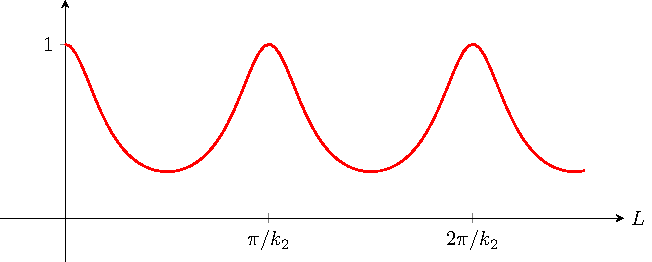
\includegraphics{images/marche_potentiel_transmission.pdf}
  \caption{Variation du coefficient de transmission de la barrière de potentiel en fonction de sa largeur. Résonnances aux multiples de $\pi/k_2$.}
\end{figure}

\subsubsection{Résolution lorsque $E < V_0$}
Une résolution similaire, voire même identique, s'obtient en posant $$k_2 \longrightarrow -i\rho_2 \qquad \rho_2 = \sqrt{2m(V_0-E)/\hbar ^2} \; \in \mathbb{R} $$ aux résultats déjà obtenus. Ainsi :
\begin{align}
  T = \left|\dfrac{A_3}{A_1}\right|^2 &= \dfrac{-4k_1 ^2 \rho_2 ^2}{-4k_1 ^2 \rho_2 ^2 + (k_1 ^2 + \rho_2 ^ 2) ^2\sin(-i\rho_2 L)} \\
  &= \dfrac{4E (V_0-E)}{4E(V_0-E) + V_0 ^2 \sinh ^ 2(\rho_2 L)}
\end{align}
Observons ce qui se passe lorsque la barrière est très imposante par rapport à l'énergie de la particule : $\rho_2L \gg 1$. Le sinus hyperbolique peut subir une approximation et la fraction peut se simplifier largement.
\begin{align}
\sinh(x) = \dfrac{e^{x} - e^{-x}}{2} &\Rightarrow \sinh^2(x)_{|_{x\gg 1}} \sim e^{2x}/4 \\
&\Rightarrow T \approx \dfrac{16(V_0-E)}{V_0 ^2} \; e^{-2\rho_2 L}
\end{align}
Nous voyons que lorsque la barrière est imposante (large et à haut potentiel), la particule a tout de même une probabilité non-nulle de la franchir. Ceci est propre à la mécanique quantique et ne serait jamais arrivé en mécanique classique. Ce phénomène porte le nom d'\textbf{Effet Tunnel} et possède comme application notable le microscope à effet tunnel.

\newpage
\section{Approximation semi-classique (WKB)}
Toujours dans le cadre de l'étude de l'équation de Schrödinger, nous allons dans cette section étudier une solution \textbf{approximative} de cette équation, valable dans la limite $\hbar \longrightarrow0$. Cette approximation est nommée en l'honneur de Léon Brillouin, Hendrik Anthony Kramers et Gregor Wentzel. L'idée est la suivante : en poussant $\hbar$ vers zéro, nous devrions retrouver des résultats de la mécanique classique. Abordons donc cela en écrivant premièrement l'équation de Schrödinger. Ensuite, inteprétons la solution obtenue.
\subsection{Résolution de l'équation de Schrödinger}

\begin{equation}\label{eq:ch2-WKB-schrod}
  -\dfrac{\hbar^2}{2m} \partial_x ^2 \phi + V(x)\psi = E\psi
\end{equation}

Posons $\psi(x) = A(x) e^{i\; S(x)/\hbar}$. Pour remplacer dans \ref{eq:ch2-WKB-schrod}, calculons d'abord les dérivées de $\psi$ en fonction de $A$ et $S$ et écrivons ce que donne l'équation de Schrödinger.
\begin{align}
  \psi' &= \left[ A' + \dfrac{i}{\hbar} S' A\right]e^{i\; S/\hbar} \\
  \psi'' &= \left[A'' + \dfrac{i}{\hbar} (S''\; A + S'\; A') - \dfrac{1}{\hbar ^2} S^{\prime 2} A + \dfrac{i}{\hbar} S' \; A'\right] e ^{i\; S/\hbar} \\
  \Rightarrow -&\dfrac{\hbar ^2 }{2m} \left[A'' + \dfrac{i}{\hbar} (S''\; A + S'\; A') - \dfrac{1}{\hbar ^2} S^{\prime 2} A + \dfrac{i}{\hbar} S' \; A'\right] e ^{i\; S/\hbar} + VA e ^{i\; S/\hbar} = EA e ^{i\; S/\hbar} \label{eq:ch2-WKB-SchrodAS}
\end{align}
En séparant les parties réelle et imaginaire de l'équation \ref{eq:ch2-WKB-SchrodAS}, on obtient le système suivant. Ce système est l'équivalent de \ref{eq:ch2-WKB-schrod}.
\begin{align}
      2S' \; A' + A \; S'' &= 0 \label{eq:ch2-WKB-SchrodAS-Im} \\
      \dfrac{S^{\prime 2}}{2m} - \dfrac{\hbar ^2}{2m} \dfrac{A''}{A} + V &= E \label{eq:ch2-WKB-SchrodAS-Re} 
\end{align}
L'équation \ref{eq:ch2-WKB-SchrodAS-Im} a une solution exacte. Elle est donnée par 
\begin{equation}
  A(x) = \dfrac{A_0}{\sqrt{S'(x)}}
\end{equation}
L'équation \ref{eq:ch2-WKB-SchrodAS-Re} peut être modifiée par notre approximation $\hbar \longrightarrow 0$, car alors $\hbar ^2/2m \longrightarrow 0$. L'équation obtenue est \textbf{l'équation de Hamilton-Jacobi}\footnote{Retenez bien ce nom car il m'a valu 4 points sur 20 à l'examen de Mécanal}.
\begin{equation}
  \dfrac{S^{\prime 2}}{2m} + V(x) = E
\end{equation}
En posant $p(x) = \sqrt{2m[E - V(x)]}$, on obtient aisemment
\begin{equation}
  S(x) = \pm \int ^x d x' p(x')
\end{equation}
Et la fonction d'onde prend alors la forme suivante :
\begin{equation} \label{eq:ch2-WKB-solution}
  \psi(x) = \pm \dfrac{A_0}{\sqrt{p(x)}} e^{\pm i \; \int ^x d x' p(x')/\hbar}
\end{equation}

\subsection{Interprétation de la solution}

\subsubsection{La vitesse de groupe du paquet d'onde est la vitesse classique}
L'impulsion de la particule est donnée par la fonction $p$. Calculons le nombre d'onde par la relation de De Broglie pour le nombre d'onde. Ce résultat sera important pour obtenir la vitesse de groupe. Il est important de saisir ici que le nombre d'onde dépend de la position.
$$k(x) = \dfrac{p(x)}{\hbar}$$
La vitesse de groupe $v_g$ est donnée par $d\omega/d k$. Alors on fait les physiciens et on renverse la fraction pour dériver $k$ par rapport à $\omega$ qu'on exprime comme $E/\hbar$. Alors :
$$\dfrac{1}{v_g} = \dfrac{d k}{d \omega} = \dfrac{d (p/\hbar)}{E/\hbar} = \dfrac{d p }{d E} = \dfrac{m}{p(x)}=  \dfrac{1}{v_{\text{classique}}}$$
Ainsi, nous voyons que l'approximation semi-classique mène à une solution de l'équation de Schrödinger qui, une fois utilisée pour construire des paquets d'onde pour constituer une particule, donne une vitesse de groupe égale à la vitesse classique de la particule.

\subsubsection{Région classiquement permise et région classiquement interdite}
La région classiquement permise est définie par l'ensemble des $x$ où $V(x) < E$. Dans cette région, on peut voir par la forme \ref{eq:ch2-WKB-solution} de la fonction d'onde que la probabilité de présence de la particule est inversement proportionnelle à l'impulsion. Ceci est le cas car pour $E>V$, $p\in \mathbb{R}$ donc l'exponentielle dans \ref{eq:ch2-WKB-solution} reste imaginaire donc son module reste 1. On voit alors que la probabilité de présence diminue quand l'impulsion de la particule augmente, ce qui rejoint notre intuition\footnote{De toute façon quand ça parle de mécanique classique, tout rejoint un peu notre intuition.}.
\begin{center}
  Région classiquement permise : $E>V(x) \quad \Rightarrow \quad |\psi|^2 \propto \dfrac{1}{p}$
\end{center}

Dans la zone interdite, $E<V$ et l'impulsion devient alors imaginaire. L'exponentielle devient réelle et la probabilité de présence devient proportionnelle à une exponentielle négative, mais pas nulle ! On retrouve ici l'effet tunnel déjà discuté, mais ici pour un potentiel quelconque qui est supérieur à l'énergie. Attention : on ne retrouve que l'exponentielle négative car les considérations physiques (fonction d'onde bornée) imposent un coefficient nul à l'exponentielle croissante (pour éviter qu'elle explose à l'infini).
\begin{center}
  Région classiquement interdite : $E<V(x) \quad \Rightarrow \quad |\psi|^2 \propto e^{-\int ^x p(x') d x'}$
\end{center}

Les figures ci-dessous reprennent un cas de potentiel et l'allure de la fonction d'onde correspondante. On voit aux lignes verticales pointillées, qui correspondent aux frontières entre les régions permise et interdite, que la probabilité devient exponentiellement décroissante mais non nulle (effet tunnel).
\begin{figure}[h]
  \centering
  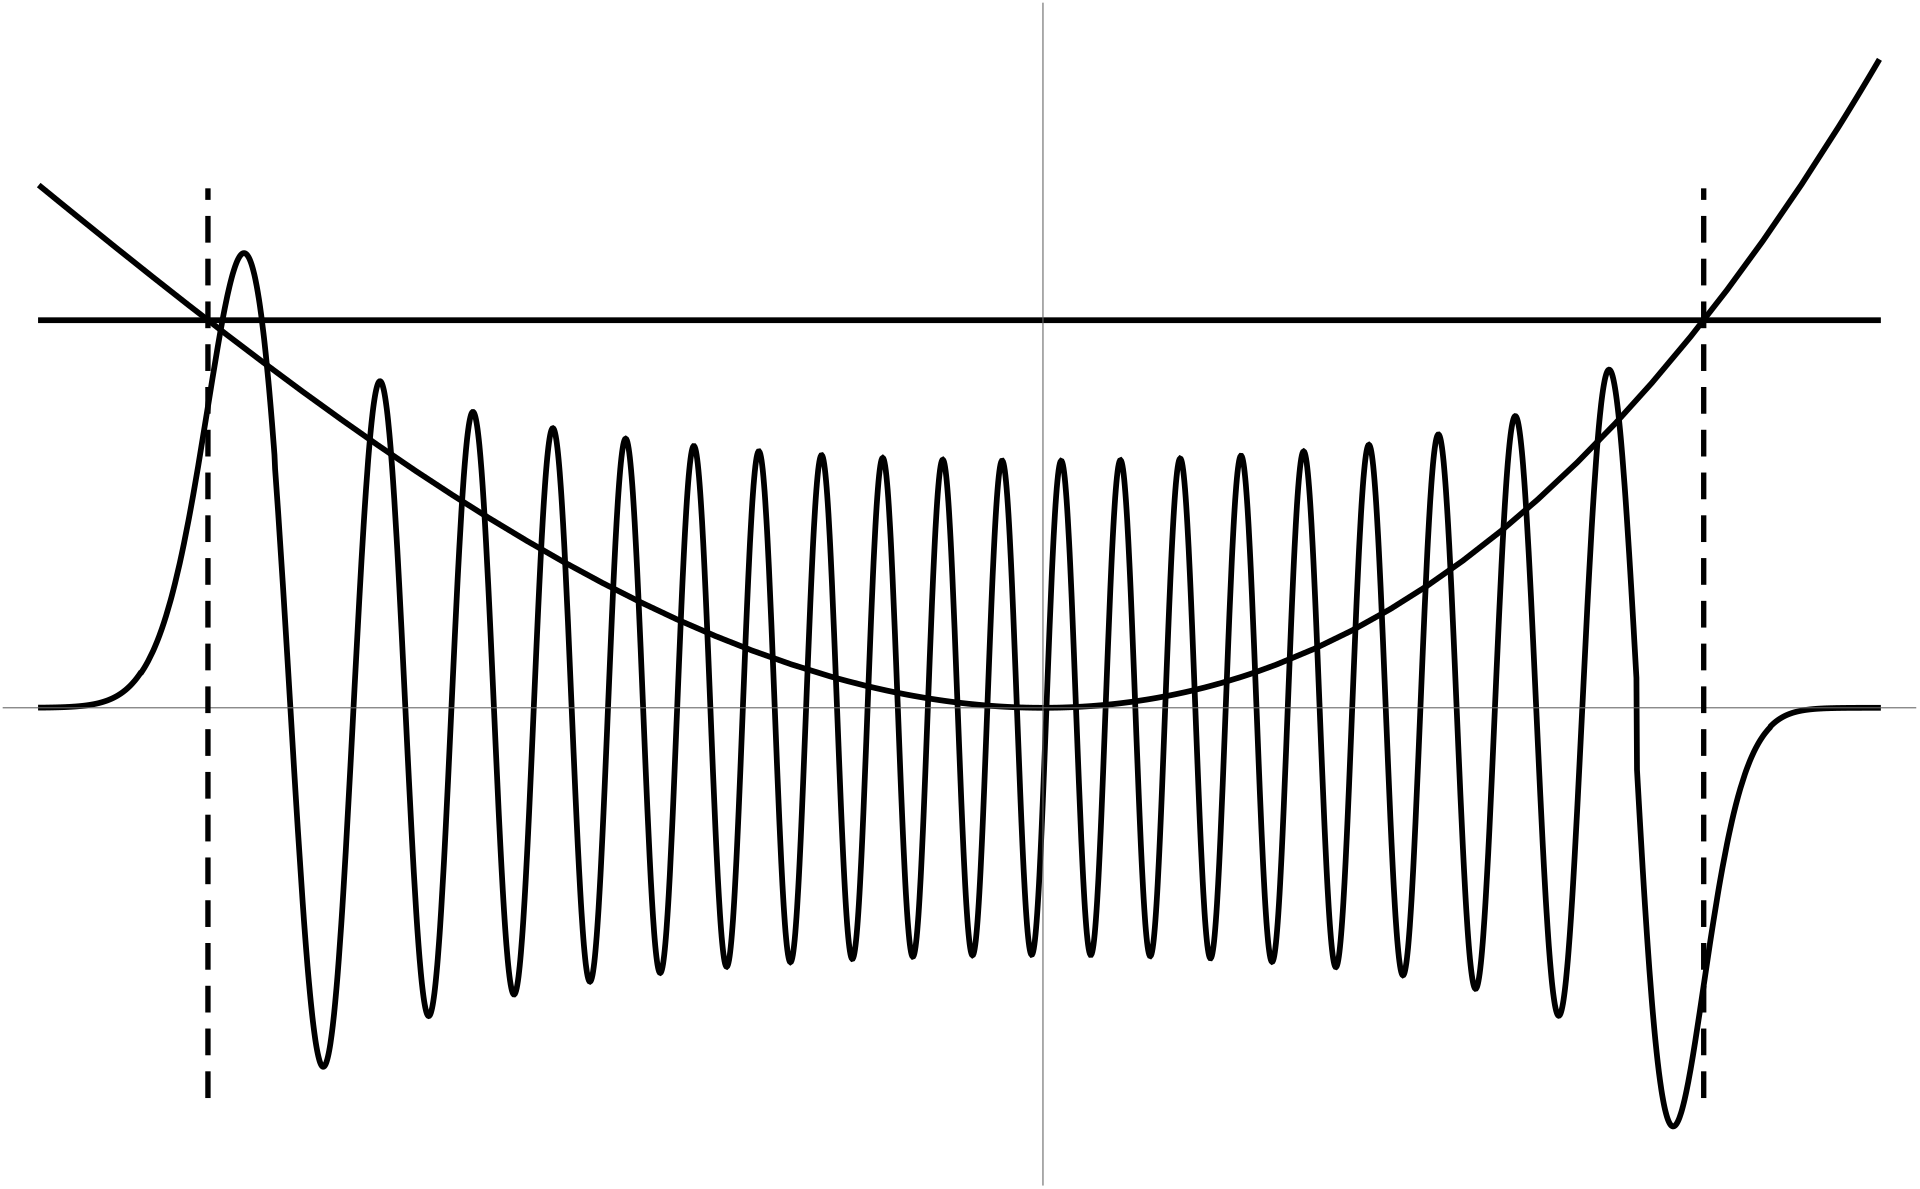
\includegraphics[width=.4\linewidth]{images/WKB_approximation_example.svg.png} \\ 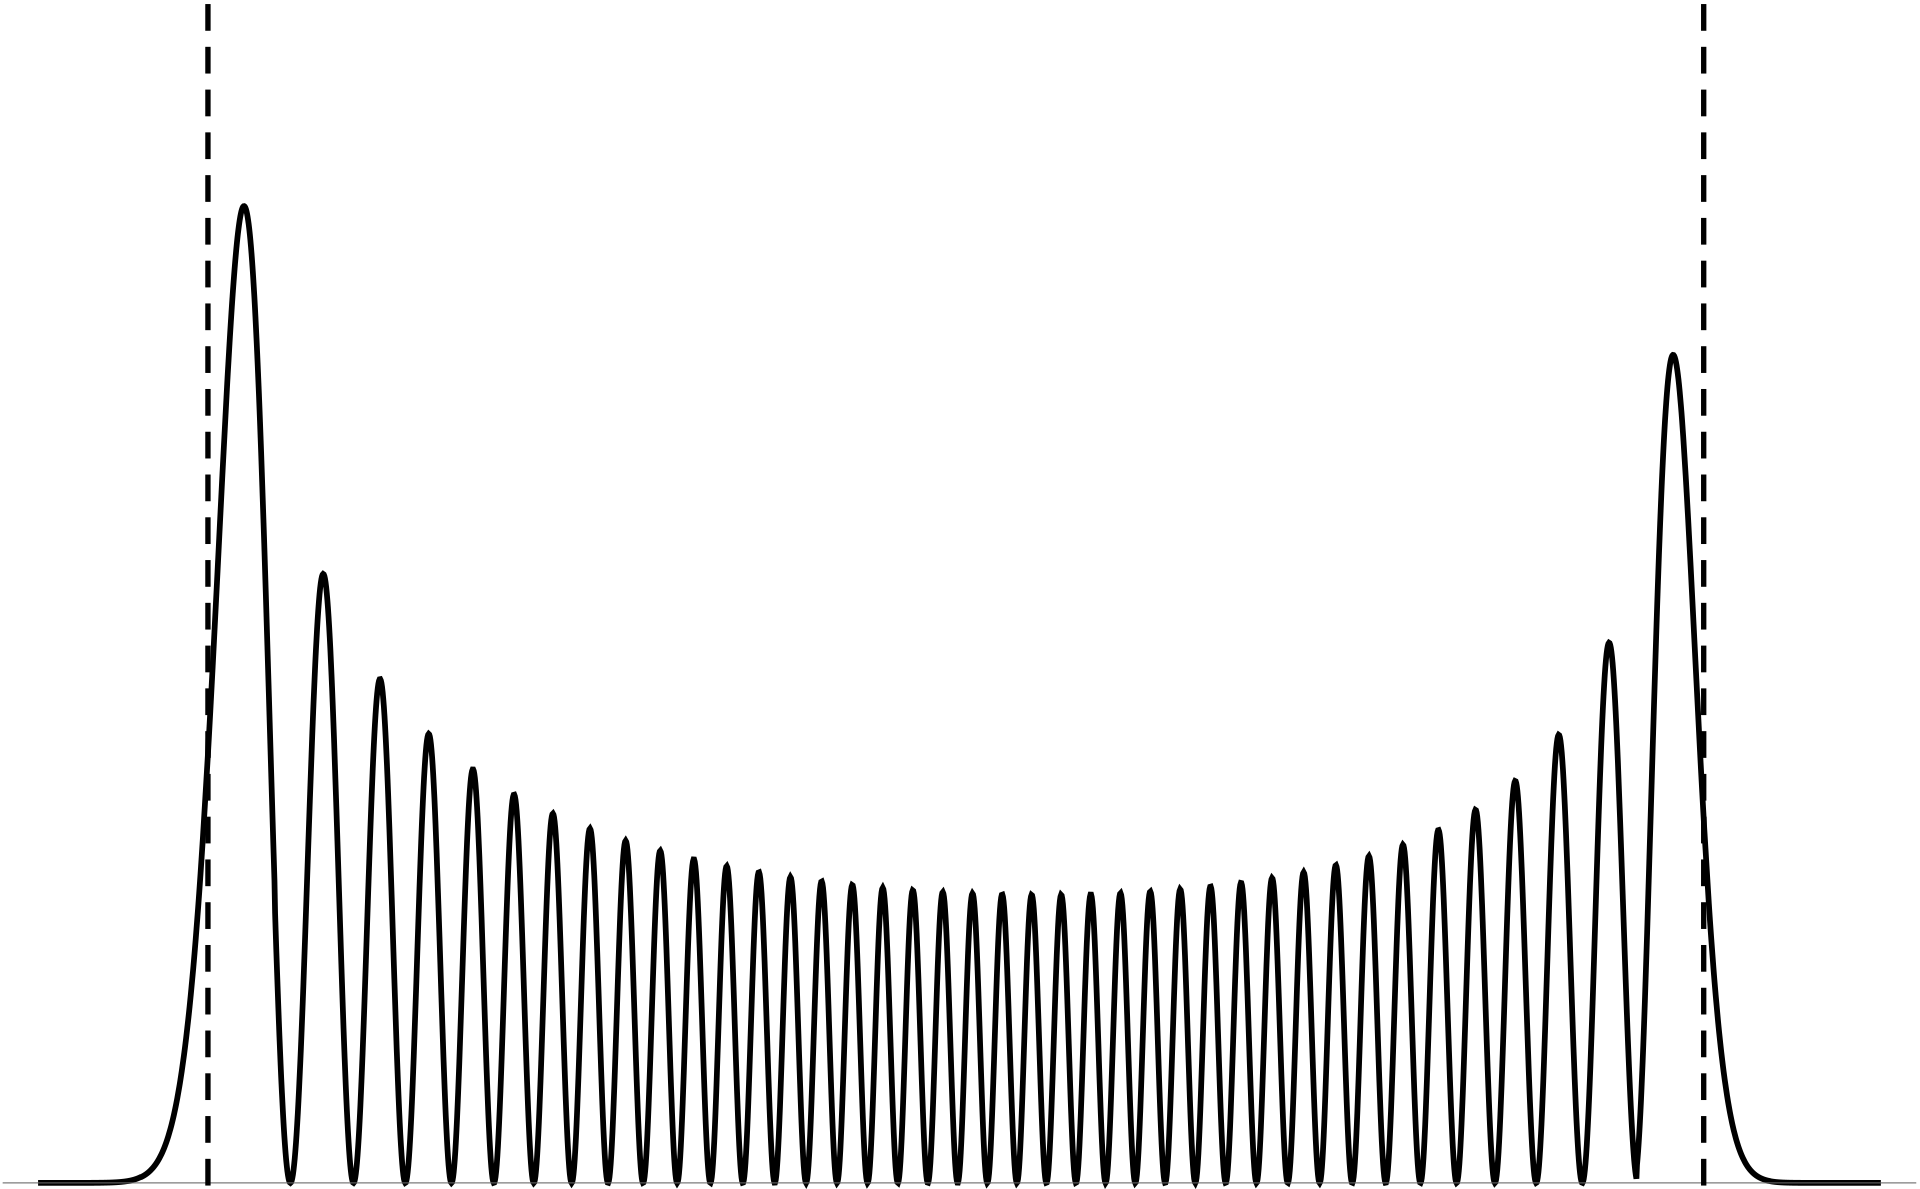
\includegraphics[width=.4\linewidth]{images/WKB_approximation_example_2.svg.png}
  \caption{Graphe d'une fonction d'onde d'une particule et de sa densité de probabilité de présence sous l'approximation WKB.}
\end{figure}

\subsubsection{Etats liés}
Si nous sommes dans le cas d'une solution qui décroit exponentiellement à grande distance, en notant $b$ et $a$ les points de rebroussement de la trajectoire classique, les états liés, dans la région permise donc, sont décrits par les fonctions suivantes, selon si on est proche de la frontière gauche avec la région interdite ou la frontière droite :
\begin{equation}
  \begin{array}{llr}
    \psi(x) &= \dfrac{1}{\sqrt{k(x)}} \; \cos\left[\int_b ^x k(x')\; d x' \quad - \pi/4\right] & x>b \\   
    \psi(x) &= \dfrac{1}{\sqrt{k(x)}} \; \cos\left[\int_x ^a k(x')\; d x' \quad + \pi/4\right] & x<a    
  \end{array}
\end{equation}
Une condition de quantification est que la somme des phases des cosinus soit égale à un multiple de $\pi/2$ \bf{confirmation needed, source wikipedia}. En sommant sur le domaine d'intégration, on obtient l'intégrale du nombre d'onde entre les deux points de rebroussement (les points de frontière).
\begin{center}
  Condition de quantification semi-classique : $\dfrac{1}{\hbar} \int_b ^a dx \sqrt{2m(E-V(x))} \quad = \left(n+\dfrac{1}{2}\right) \pi$
\end{center}

\subsection{Application de l'approximation WKB en physique nucléaire}
Par la section précédente, nous avons compris que l'approximation WKB consistait à prendre la limite $\hbar \to 0$, mais dans quel cas pouvons-nous réellement passer à une application de cette approximation? \\
{\color{red}{Tentative d'explication mais le paragraphe en entier est à vérifier :}} Il se trouve que cette approximation peut être valable lorsque l'on veut considérer des effets quantiques qui s'appliquent sur un système, pendant que ce dernier peut également être décrit d'un point de vue classique, 
ainsi que lorsqu'il n'est pas possible de trouver de solution analytique sans faire aucune approximation. \\

Nous allons ici illustrer un exemple d'application de l'approximation WKB qui est celui de la désintégration-$\alpha$, et qui en particulier
met en avant la loi de Geiger-Nuttal. \\
Nous allons prendre en compte le fait que des particules $\alpha$ vont s'échapper d'un noyau par \textit{effet tunnel}, et notre description fera apparaître des \textit{interprétations probabilistes} sur l'émission de ces particules, 
tout en utilisant les relations données par l'approximation WKB afin d'en tirer une conclusion cohérente avec des données expérimentales. \\

Avant de rentrer dans les détails, rappelons brièvement ce que sont la désintégration alpha et un temps de demi-vie $t_{1/2}$: 
\begin{itemize}%[label = \textbullet]
  \item \textbf{Désintégration $\alpha$} $\equiv$ (wikipédia {\color{red}{à vérifier}}) forme de désintégration radioactive où un noyau atomique éjecte une particule $\alpha$
  ( $= He^{++}$) et se transforme en un noyau plus léger ; 
  \item \textbf{Demi-vie $t_{1/2}$} d'un isotope radioactif $\equiv$ (wikipédia) c'est le temps au bout duquel la moitié des noyaux de cet isotope initiaux se sont désintégrés. \\
  Notons qu'il est important de reconnaître la différence entre cette définition et celle d'un temps moyen : 2 fois le temps de demi-vie $\ne$ la vie complète!!  
\end{itemize}

Rentrons à présent dans des détails de calculs. \\
Considérons un noyau de rayon $R$ qui contient des particules $\alpha$ possédant une énergie $E$. 
Les particules $\alpha$ sont confinées dans le noyau, autrement dit leur énergie est plus faible que le potentiel qui les retient.
Or, nous avons déjà vu qu'une particule pouvait traverser une zone classiquement interdite par effet tunnel, et se propage comme une onde "evanescente" (qui décroît exponentiellement) dans cette zone. \\
C'est en fait ce qu'il va se passer ici pour les particules $\alpha$ ; on peut, analogiquement, imaginer que les particules sont confinées dans une boîte, faisant des allers-retours. C'est à ces points de rebroussement que peut se produire la transmission de particules par effet tunnel. \\

Une fois sorti du noyau, le potentiel ressenti par les particules $\alpha$ est simplement le potentiel coulombien créé par les charges du noyau. Ainsi, pour tout $r > R$, le potentiel s'écrit comme suit :
\begin{equation}
  V(r) = \frac{z_{\alpha} z e^2}{4 \pi \epsilon_0 r} %pour un potentiel crée par une charge z, on ne devrait pas avoir juste z dans cette expression au lieu de z_alpha *z ?
\end{equation}
où $z_{\alpha}$, $z$ $\equiv$ charges du noyau. \\
%+ graphe qui illustre le potentil vu par les particules alpha

Notons $R_{\alpha}$ la distance à partir de laquelle l'énergie $E$ de la particule devient plus grande que le potentiel coulombien ressenti $V(r)$, autrement dit, $R_{\alpha}$ est la distance au noyau à partir de laquelle la particue devient libre et peut se propager de manière semi-classique (c'est-à-dire tel que la longueur d'onde varie très peu sur une distance égale à la longueur d'onde même). \\
L'énergie de la particule étant considérée comme une constante dans ce cas-ci, et puisque l'on considère également que la particule $\alpha$ émise peut se propager au moins jusqu'à une distance $R_{\alpha}$ du noyau, notons son énergie $E$ : $$ E= \frac{z_{\alpha}z e^2}{4 \pi \epsilon_0 R_{\alpha}}$$ 
Ensuite, il se trouve que la probabilité d'émission de particule alpha par unité de temps se trouve approximativement par l'inverse du temps de demi-vie. Cela illustre bien le fait que plus ce temps de demi-vie est long, moins il n'y a de probabilité qu'une particule alpha soit émise en une seconde. En utilisant les relations de la fonction d'onde obtenues grâce à l'approximation WKB,
nous avons en particulier que : 
\begin{align}
  \frac{P( \mbox{ émission } )}{temps} \approx \frac{1}{t_{1/2}} \approx e^{-2 \gamma} \quad \mbox{ ($\approx \lvert \psi (r) \rvert ^2$ effet tunnel) } 
\end{align}
où  \begin{align*}
  \gamma &= \frac{1}{\hbar} \int_R^{R_{\alpha}} \sqrt{2 m_{\alpha} (V(r) - E)} dr \\
  &= \frac{1}{\hbar} \sqrt{2 m_{\alpha}} \sqrt{\frac{z_{\alpha} z e^2}{4 \pi \epsilon_0}} \int_R^{R_{\alpha}} \sqrt{\frac{1}{r} - \frac{1}{R_{\alpha}}} dr \\
  &= \frac{1}{\hbar} \sqrt{2 m_{\alpha}} \sqrt{\frac{z_{\alpha} z e^2}{4 \pi \epsilon_0}} \int_R^{R_{\alpha}} \frac{1}{\sqrt{R_{\alpha}}} \sqrt{\frac{R_{\alpha}}{r} - 1} dr \\
  &= \frac{1}{\hbar} \sqrt{2 m_{\alpha}} \sqrt{\frac{z_{\alpha} z e^2}{4 \pi \epsilon_0}} \sqrt{R_{\alpha}} \int_0^1 \sqrt{\frac{1-z}{z}} dz \quad \mbox{ (grâce au changement de variable : $z = \frac{r}{R_{\alpha}}$)} \\
  &\approx \frac{\pi}{2} \sqrt{R_{\alpha}} \quad \mbox{ (intégrale calculée par un changement de variable comme $z = cos^2(x)$ par exmple)} 
\end{align*}

Enfin, en utilisant le fait que $R_{\alpha} = \frac{z_{\alpha} z e^2}{4 \pi \epsilon_0 E}$, on a :
\begin{align}
\label{Loi de Geiger-Nuttal}
  \gamma &= \frac{\pi}{2 \hbar} \sqrt{2 m_{\alpha}} \left( \frac{z_{\alpha} z e^2}{4 \pi \epsilon_0} \right) \frac{1}{\sqrt{E}} \notag \\
  \implies & log(t_{1/2}) = a \frac{z}{\sqrt{E}} + b \quad \mbox{ \textbf{Loi de Geiger-Nuttal}} 
\end{align}

\bf{Remarque : }{\begin{itemize}
  \item Nous pouvons voir que cette équation \ref{Loi de Geiger-Nuttal} met en relation l'inverse de la racine de l'énergie au logarithme du temps de demi-vie.
  Cela signifie qu'une grande augmentation du temps $t_{1/2}$ est équivalent à une légère diminution de l'énergie. On peut donc considérer que des isotopes qui émettent des particules alpha, à un temps de demi-vie d'ordres de grandeur assez variés, ont approximativement la même énergie ;
  \item Cette loi est bien vérifiée expérimentalement ;
  \item Elle explique également pourquoi la désintégration en noyau plus lourd est impossible (dépendance en $m_{\alpha}$ et $z_{\alpha}$) {\color{red}{Pourquoi???}}
\end{itemize}
}

\end{document}

%Ajout schéma de Massar : graphes des données expérimentales 
